\documentclass[11pt,a4paper]{article}

\usepackage{graphicx}
\usepackage{mathtools,amssymb}

\usepackage{amsthm}
\theoremstyle{definition}
\newtheorem{definition}{Definition}[section]

\usepackage{enumitem}
\usepackage{float}
\usepackage[number-unit-product = {\ }]{siunitx}

\usepackage[CJKmath=true,AutoFakeBold=3,AutoFakeSlant=.2]{xeCJK}
\setCJKmainfont{標楷體}
\setCJKsansfont{微軟正黑體} 
\setCJKmonofont{標楷體}
\newCJKfontfamily\Kai{標楷體}       
\newCJKfontfamily\Hei{微軟正黑體}   
\newCJKfontfamily\NewMing{新細明體} 
\XeTeXlinebreaklocale "zh"

\usepackage[backend=biber, style=numeric, sorting=none]{biblatex}
\addbibresource{references.bib} % 告訴 LaTeX 參考資料檔案的位置

\usepackage[colorlinks=true,
    linkcolor=blue,    % 目錄和章節標題連結 = 黑色
    citecolor=blue,     % 文獻引用超連結 = 藍色
    urlcolor=blue,      % 網址超連結 = 藍色
    filecolor=blue,     % 檔案超連結 = 藍色
    anchorcolor=blue    % 其他定位點 = 藍色
]{hyperref}


\begin{document}

    \begin{titlepage}
        \centering % 頁面內容置中

        % --- 校名與報告名稱 ---
        \vspace{1cm} % 頁首留白
        {\Huge \bfseries
            國立陽明交通大學 \\
            \vspace{0.5cm}
            物理實驗結報
        }
        \vspace{2cm}
        \rule{\linewidth}{1pt} % 新增分隔線
        \vspace{2cm}

        % --- 實驗主題 ---
        {\Huge \bfseries 一維運動\par}
        \vspace{\fill} % 自動填滿垂直空間,將下方內容推至頁底

        % --- 作者與指導老師資訊 ---
        \Large % 設定以下文字大小
        \begin{tabular*}{\textwidth}{l @{\extracolsep{\fill}} l}
            系級: & 電子物理系一年級 \\
            組別: & B1-10 \\
            作者: & 114651077 簡睿均 \quad 114651018 何宇奕 \\
            指導教授:\quad & 許鈺敏 \\
            指導大助: & 詹皓喆 \\
            指導小助: & 張皓軒、陳奕安 \\
        \end{tabular*}

        \vspace{2cm} % 頁尾留白

    \end{titlepage}

    \subsection*{分工}
    \begin{enumerate}
        \item 簡睿均 50\%:撰寫結報之封面、前言、原理、方法、結果、討論、結論、參考資料、附錄。整合結報,及完成預報,繪製示意圖,共同進行實驗,並參與討論。
        \item 何宇奕 50\%:撰寫結報之方法、結果、討論、參考資料。實驗前excel表格準備,及實驗後作圖等數據分析,共同進行實驗,並參與討論。
    \end{enumerate}
    
    \section{前言}

        \subsection{實驗動機}
            牛頓的運動定律(Newton's laws of motion)和運動學(kinematics)是物理學中力學的基礎。而在日常生活中雖然很容易感受到力能對物體造成速度變化,卻難以量化。本實驗希望藉由重力拉動滑車,配合光閘精準測量加速度,驗證牛頓第二運動定律。
            
        \subsection{實驗目的}
            藉由砝碼的重力拉動水平和爬坡軌道上的滑車,驗證牛頓第二定律。本實驗包含以下三個實驗:

            \begin{enumerate}
                \item 實驗A\par
                在水平軌道上,固定拉力 $F$ ,以總質量 $M$ 對加速度倒數 $\frac{1}{a}$ 坐圖探討總質量和加速度 $a$ 的關係。
                \item 實驗B\par
                在水平軌道上,固定總質量 $M$,以加速度 $a$ 對拉力 $F$ 作圖探討總質量和加速度的關係。
                \item 實驗C\par
                在爬坡軌道上,固定拉力 $F$ 與總質量 $M$,並分析
                    \begin{enumerate}
                        \item 加速度 $a$ 對傾角 $\theta$ 作圖。
                        \item 加速度 $a$ 對 $\sin\theta$ 作圖。
                    \end{enumerate}
                探討斜坡傾角和加速度的關係。
            \end{enumerate}

        \subsection{力學演變的歷史}

            在古希臘時期,亞里斯多德認為「運動必須持續受到推力」,否則物體將會停止。這一觀點雖直覺,但卻無法解釋如拋體運動或行星運行等自然現象。到了十六世紀,伽利略透過斜面實驗與思想實驗挑戰了傳統觀點:他主張若物體在光滑無阻力的斜面上運動,則會以不減速的狀態持續滑行,藉此提出了「慣性」的概念。更進一步,他透過思想實驗指出,若將兩個斜面無限延長至水平,則物體將永遠不會停止運動,這與亞里斯多德的觀念截然相反。
            \par 有了前人的思考作為基礎,牛頓在 1687 年出版《自然哲學的數學原理 (Philosophiæ Naturalis Principia Mathematica)》\cite{newton:1687}發表經典的三大牛頓運動定律。其中,他不僅總結了伽利略的觀察,更提出了三大運動定律,融入了當時逐漸成熟的數學方法,奠定了經典力學的完整架構。雖然過程有些小錯誤,但牛頓的運動定律配合他的重力理論和由他發展的微積分技巧成功解釋克卜勒定律。

        \subsection{牛頓運動定律(Newton's laws of motion)}

        牛頓運動定律包含三個表述:
        
            \begin{enumerate}
                \item 第一定律(慣性定律):在慣性座標系下,不受力的物體恆做等速度運動。慣性定律不只闡明了物體運動的本質,更定義了慣性座標系,賦予第二定律實際的意義。
                \item 第二定律(加速度定律):在慣性座標系下,物體的質量和受力的關係為:
                \begin{equation}
                    \vec{F} = m\vec{a}
                \end{equation}
                其中$\vec{F}$為物體受淨力,$\vec{a}$為物體加速度,$m$ 為物體慣性質量。加速度定律在力學分析上不可或缺,同時定義了力的大小和慣性質量。
                \item 第三定律(作用力與反作用力定律):任何作用力必伴隨大小相等、方向相反的反作用力。作用力與反作用力定律讓物理學家得以衍生出更多理論例如:動量守恆。
            \end{enumerate}

    \section{實驗原理}

        \subsection{實驗裝置圖}
        
        \begin{figure}[H]
            \centering
            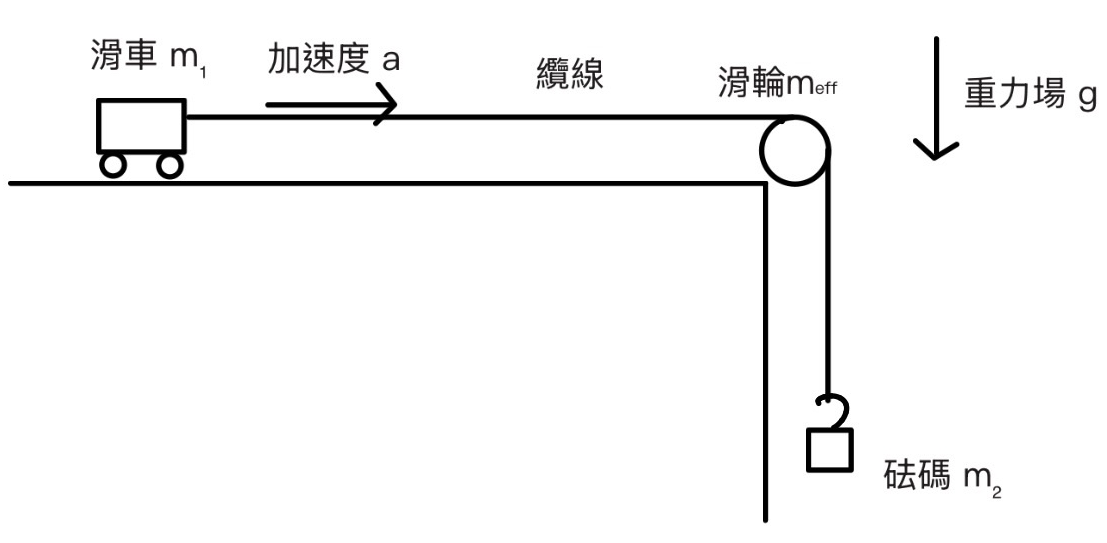
\includegraphics[width=0.8\textwidth]{水平軌道示意圖.png}
            \caption{實驗A、實驗B示意圖}
            \label{fig:實驗A、實驗B示意圖}
        \end{figure}

        \begin{figure}[H]
            \centering
            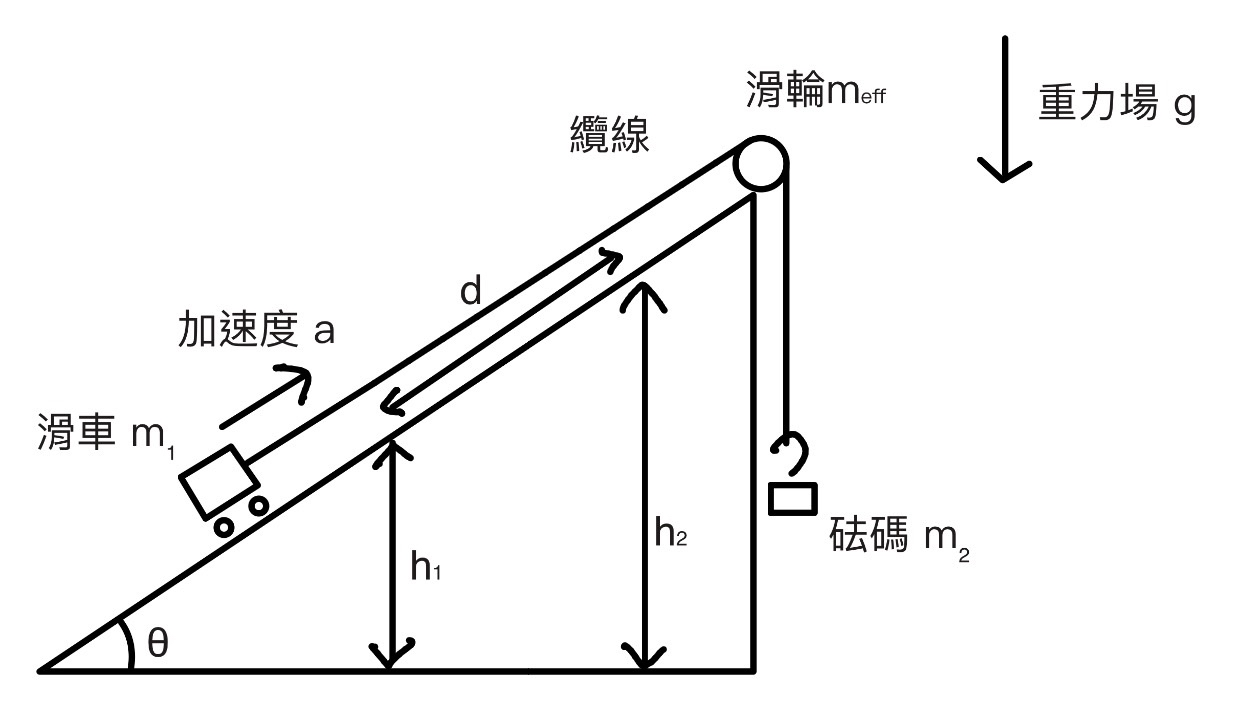
\includegraphics[width=0.8\textwidth]{斜坡示意圖.png}
            \caption{實驗C示意圖}
            \label{fig:實驗C示意圖}
        \end{figure}

        \subsection{實驗參數}
            \begin{enumerate}
                \item 滑輪質量 $m_1$ 與砝碼質量 $m_2$ 由電子秤量測。
                \item 軌道高度 $h_1, h_2$ 由直尺量測。
                \item 距離 $d$ 由軌道上標尺量測。
                \item 加速度 $a$ 由軟體監測光閘測量滑輪轉速取得。
                \item 滑輪等效質量 $m_{eff}$ 已知為 \SI{4.50}{\gram}。
                \item 重力加速度為 \SI{9.7890191}{\meter\per\second\squared},此數值由國土測繪中心網站取得 \cite{nlsc:twd97}。
                \item 總質量 $M = m_1 + m_2 + m_{eff}$。
                \item 軌道傾角 $\theta$ 由 $h_1, h_2, d$ 經反三角函數計算。
                \item 拉力由砝碼和滑車重力沿位移方向的分力計算。
            \end{enumerate}

        \subsection{公式推導}
            \begin{enumerate}

                \item 滑輪等效質量推導\par
                參考 \autoref{fig:實驗C示意圖},設砝碼相對於初始點之向下位移為 $y$,砝碼速率為$v$,滑輪半徑為$r$,滑輪沿圓心轉動慣量為 $I$,則力學能為

                \begin{gather}
                    m_1 g (-y)\sin{\theta} + m_2 g (-y) + \frac{1}{2}(m_1 + m_2)v^2 + \frac{1}{2}I(\frac{v}{r})^2
                \end{gather}

                在不考慮摩擦力的情況,力學能守恆,式(2)對時間微分應為0:

                \begin{gather}
                    m_1 g \sin{\theta} v + m_2 g v + (m_1 + m_2 + \frac{I}{r^2})av
                \end{gather}                

                將 $F = m_2g + m_1g \sin{\theta}$帶入化簡得

                \begin{gather}
                    F = (m_1 + m_2 + \frac{I}{r^2})a
                \end{gather}

                令等效質量 $\displaystyle m_{eff} = \frac{I}{r^2}$ ,則(4)可改為牛頓第二定律的一般形式

                \begin{gather}
                    F = (m_1 + m_2 + m_{eff})a
                \end{gather}

                對於實驗A、實驗B,可視為 $\theta = 0$,結果相同

                \item 實驗A的數據分析\par
                參考 \autoref{fig:實驗A、實驗B示意圖},根據式(5)的推導,將$F = m_2g$ 帶入得

                \begin{gather}
                    m_2g = (m_1 + m_2 + m_{eff})a
                \end{gather}

                將 $M = (m_1 + m_2 + m_{eff})$帶入經移項得

                \begin{gather}
                    \frac{1}{a} = \frac{M}{m_2g}
                \end{gather}                

                則由$\displaystyle\frac{1}{a}$對總質量 $M = m_1 + m_2 + m_{eff}$ 作圖理論上應得到過原點斜率為 $F = \displaystyle\frac{1}{m_2 g}$的斜直線。                

                \item 實驗B的數據分析\par
                參考 \autoref{fig:實驗A、實驗B示意圖},根據式(5)的推導
                
                \begin{gather}
                    a = \frac{F}{m_1 + m_2 + m_{eff}}
                \end{gather}

                則由加速度 $a$ 對拉力 $F = m_2g$ 作圖理論上應得到過原點斜率為 $\displaystyle{\frac{1}{m_1 + m_2 + m_{eff}}}$的斜直線。

                \item 實驗C的數據分析\par
                參考 \autoref{fig:實驗C示意圖},根據式(5)的推導,將$F = m_2g + m_1g \sin{\theta}$ 帶入得

                \begin{gather}
                    - m_1 \sin{\theta} g + m_2 g = (m_1 + m_2 + m_{eff}) a
                \end{gather}

                移像得

                \begin{gather}
                    a = \frac{- m_1 g \sin{\theta} + m_2 g}{m_1 + m_2 + m_{eff}}
                \end{gather}

                則由加速度 $a$ 對 $\sin{\theta}$ 作圖理論上可得斜率為\par$\displaystyle\frac{- m_1}{m_1 + m_2 + m_{eff}}$,截距為 $\displaystyle\frac{m_2 g}{m_1 + m_2 + m_{eff}}$ 的斜直線。

                當 $\theta < \ang{10}$ , $\sin{\theta} \approx \theta$。式(9)可再簡化為

                \begin{gather}
                    a = \frac{- m_1 g \theta + m_2 g}{m_1 + m_2 + m_{eff}}
                \end{gather}

                則由加速度 $a$ 對軌道傾斜角度 $\theta$ 作圖理論上可得接近一斜率為\par$\displaystyle\frac{- m_1}{m_1 + m_2 + m_{eff}}$,截距為 $\displaystyle\frac{m_2 g}{m_1 + m_2 + m_{eff}}$的斜直線。

                本實驗以測量長度 $d、h_1、h_2$ 以提升精確度,其關係式為 $\sin\theta = \displaystyle\frac{h_2 - h_1}{d}$,亦即 $\theta = \sin ^{-1}\left(\displaystyle\frac{h_2 - h_1}{d}\right)$。
            \end{enumerate}

    \section{實驗方法(含避免誤差之方法及校正)}

        \subsection{實驗儀器}

            鋁製軌道、滑車、水平儀、軌道斜面支架、掛鉤、砝碼、細線、直尺、電子秤、含滑輪之光閘(含連接線)、數位轉接頭(PS-2159),藍芽訊號收發器(PS-3200)、電腦(含Capstone程式軟體)

        \subsection{水平軌道實驗步驟(實驗A、實驗B)}

            \begin{enumerate}

                \item 將實驗裝置架設如 \autoref{fig:實驗A、實驗B示意圖}。
                \item 將水平儀置於軌道上如 \autoref{fig:水平儀校正}。調整軌道下方螺絲使氣泡在兩黑線之間,以確保軌道為水平。
                \item 修正棉線長度,使當滑車於軌道離滑輪最遠處處時,砝碼離地面最遠,以確保滑車可以移動最遠距離,增加樣本數,減少實驗誤差。
                \item 將軟墊置於砝碼正下方,避免砝碼下落時造成破壞及噪音。
                \item 將砝碼垂吊及置於滑車上以調整重量,並用電子秤歸零後測量 $m1$ 及 $m2$。
                \item 將滑車拉至軌道離最遠處,並確認砝碼沒有晃動。
                \item 於電腦軟體啟用滑輪速率監測,並放開滑車。
                \item 選取電腦軟體紀錄包含在斜直線中之數據,使用自動回歸功能得出加速度。
                \item 重複步驟5.至8.,固定砝碼質量 $m_2$ ,藉由改變滑車上砝碼質量改變 $m_1$ 
                \item 將步驟8.之結果以 $\displaystyle\frac{1}{a}$ 對 $M = m_1 + m_2 + m_{eff}$ 作圖,並與預期結果比較,作為實驗A之結果。
                \item 重複步驟5.至8.,並每次將滑車上一個砝碼移除並增加至垂吊的砝碼中,以在總質量 $M$ 不變的同時改變 $F$。
                \item 將步驟11.之結果以 $\displaystyle a$ 對 $F = M_2g$ 作圖,並與預期結果比較,作為實驗B之結果。

            \end{enumerate}

            \begin{figure}[H]
                \centering
                \includegraphics[width=0.8\textwidth]{水平儀校正.png}
                \caption{水平儀校正}
                \label{fig:水平儀校正}
            \end{figure}
        
        \subsection{傾斜軌道實驗步驟(實驗C)}

            \begin{enumerate}

                \item 將實驗裝置架設如 \autoref{fig:實驗C示意圖}。
                \item 將水平儀置於軌道上如。調整軌道下方螺絲使氣泡在兩黑線之間,以確保軌道在垂直於軌道方向沒有傾斜。
                \item 修正棉線長度,使當滑車於軌道離滑輪最遠處處時,砝碼離地面最遠,以確保滑車可以移動最遠距離,增加樣本數,減少實驗誤差。
                \item 將軟墊置於砝碼正下方,避免砝碼下落時造成破壞及噪音。
                \item 將砝碼垂吊及置於滑車上以調整重量,並用電子秤歸零後測量 $m1$ 及 $m2$。
                \item 以直尺測量 $h_1、h_2$ 並以軌道上之標尺測量 $d$。
                \item 將滑車拉至軌道離最遠處,並確認砝碼沒有晃動。
                \item 於電腦軟體啟用滑輪速率監測,並放開滑車。
                \item 選取電腦軟體紀錄包含在斜直線中之數據,使用自動回歸功能得出加速度。
                \item 重複步驟5.至9.,固定砝碼質量 $m_2$,藉由改變滑車上砝碼質量改變 $m_1$。 
                \item 將步驟8.之結果以加速度 $a$  對 $\sin{\theta}$ 作圖,並與預期結果比較。
                \item 將步驟8.之結果以加速度 $a$  對 $\theta$ 作圖,並與預期結果比較。

            \end{enumerate} 

    \section{實驗結果}
        \subsection{實驗A}

            \begin{table}[H]
                \centering
                \caption{實驗A數據表}
                \label{tab:expA_data}
                \begin{tabular}{|c|c|c|c|c|}
                    \hline
                    $m_1$ (\si{\kilogram}) &  $a$ (\si{\meter\per\second\squared}) & $1/a$ (\si{\second\squared\per\meter}) & $M$ (\si{\kilogram}) \\
                    \hline
                    0.3734 & 2.68 & 0.373 & 0.5240 \\ \hline
                    0.3832 & 2.64 & 0.379 & 0.5338 \\ \hline
                    0.3935 & 2.59 & 0.386 & 0.5441 \\ \hline
                    0.4037 & 2.55 & 0.392 & 0.5543 \\ \hline
                    0.4135 & 2.49 & 0.402 & 0.5641 \\ \hline
                    0.4335 & 2.40 & 0.417 & 0.5841 \\ \hline
                    0.4435 & 2.37 & 0.422 & 0.5941 \\
                    \hline
                \end{tabular}
            \end{table}
            
            $m_2$ 固定為\SI{0.1461}{\kilogram}

            \begin{figure}[H]
                
                \centering
                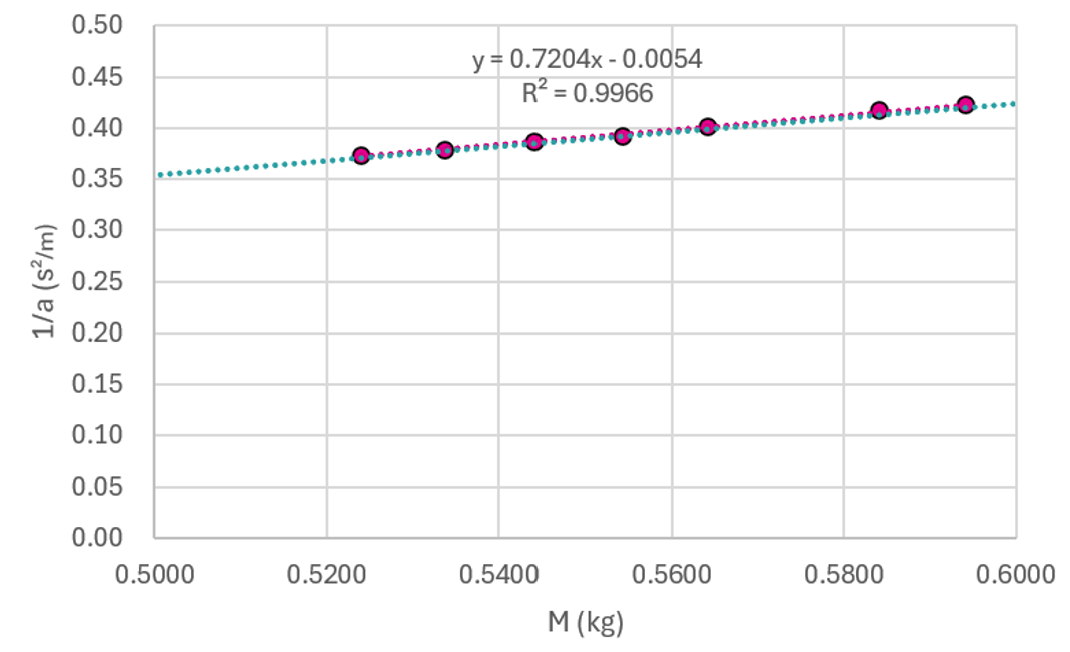
\includegraphics[width=0.8\textwidth]{實驗A數據圖.png}
                \caption{加速度倒數$\displaystyle\frac{1}{a}$與系統總質量$M$的關係圖}
                \label{fig:實驗A數據圖}

            \end{figure}

            在\autoref{fig:實驗A數據圖}中,粉紅色虛線為實際值趨勢線,藍色虛線為理論值趨勢線,其關係式如下:
            \begin{equation}
                \frac{1}{a} = \frac{M}{m_2 g} \label{eq:theory_A}
            \end{equation}

            \par 由回歸直線得出
            $\displaystyle\frac{1}{a}$ 與 $M$ 成正比,並由回歸直線得斜率 
            \par$\displaystyle{\frac{1}{m_2 g}} = $ \SI{0.7204}{\second\squared\per\kilogram\per\meter}。

        \subsection{實驗B}

            \begin{table}[H]
                \centering
                \caption{實驗B數據表}
                \label{tab:expB_data}
                \begin{tabular}{|c|c|c|c|}
                    \hline
                    $m_2$ (\si{\kilogram}) &  $F$ (\si{\newton}) & $a$ (\si{\meter\per\second\squared}) \\
                    \hline
                    0.0563 & 0.551 & 1.01 \\ \hline
                    0.0664 & 0.650 & 1.20 \\ \hline
                    0.0765 & 0.749 & 1.38 \\ \hline
                    0.0866 & 0.848 & 1.57 \\ \hline
                    0.0967 & 0.947 & 1.76 \\ \hline
                    0.1068 & 1.045 & 1.94 \\ \hline
                    0.1163 & 1.138 & 2.10 \\ \hline
                \end{tabular}
            \end{table}
            總質量 $M$ 固定為 \SI{0.5345}{\kilogram}。

            \begin{figure}[H]
                
                \centering
                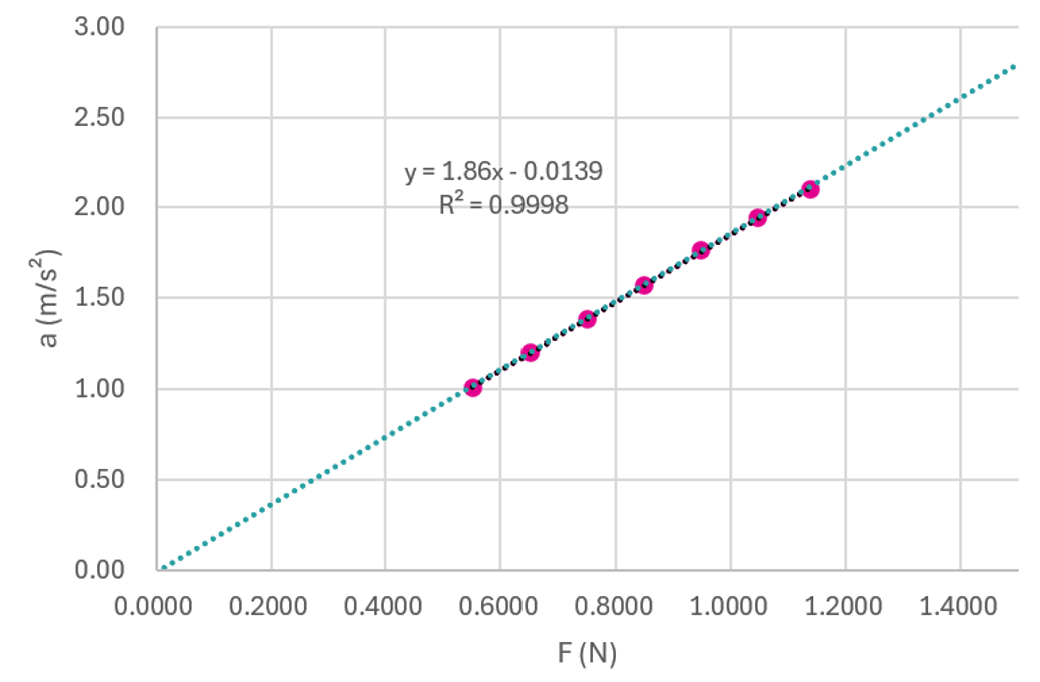
\includegraphics[width=0.8\textwidth]{實驗B數據圖.png}
                \caption{加速度$\displaystyle{a}$與拉力$F = m_2 g$的關係圖}
                \label{fig:實驗B數據圖}

            \end{figure}            

            在 \autoref{fig:實驗B數據圖}中,粉紅色虛線為實際值趨勢線,藍色虛線為理論值趨勢線,其關係式如下:
            \begin{equation}
                a = \frac{F}{m_1 + m_2 + m_{eff}} \label{eq:theory_B}
            \end{equation}

            \par 由回歸直線得出
            $a$ 與 $F$ 成正比,並由回歸直線得斜率 $\displaystyle{\frac{1}{M}} = $ \SI{1.86}{\per\kilogram}。

        \subsection{實驗C}

            \begin{table}[H]
                \centering
                \caption{實驗C數據圖}
                \label{tab:expC_data}
                \begin{tabular}{|c|c|c|c|c|}
                    \hline
                    $h_1$ (\si{\meter}) & $h_2$ (\si{\meter}) & $a$ (\si{\meter\per\second\squared}) & $\sin\theta$ & $\theta$ (\si{\radian}) \\
                    \hline
                    0.0000 & 0.0000 & 2.55 & 0.0000 & 0.0000 \\ \hline
                    0.0943 & 0.1130 & 2.46 & 0.0187 & 0.0187 \\ \hline
                    0.0962 & 0.1635 & 2.08 & 0.0675 & 0.0676 \\ \hline
                    0.0951 & 0.1255 & 2.34 & 0.0305 & 0.0305 \\ \hline
                    0.0955 & 0.1400 & 2.25 & 0.0445 & 0.0445 \\ \hline
                    0.0975 & 0.1722 & 1.99 & 0.0747 & 0.0748 \\ \hline
                    0.0993 & 0.2020 & 1.83 & 0.1027 & 0.1029 \\ \hline
                    0.1000 & 0.2252 & 1.68 & 0.1252 & 0.1255 \\ \hline
                    0.1010 & 0.2498 & 1.51 & 0.1488 & 0.1494 \\ \hline
                \end{tabular}
            \end{table}
            滑車質量 $m_1$ 固定為 \SI{0.3730}{\kilogram},掛鉤上砝碼質量 $m_2$ 固定為 \SI{0.1364}{\kilogram},軌道長度 $d$ 固定為 \SI{1.0000}{\meter}。第一筆數據以水平儀校正視為水平,無$h_1 - h_2$之有效位數問題。

            \begin{figure}[H]
                
                \centering
                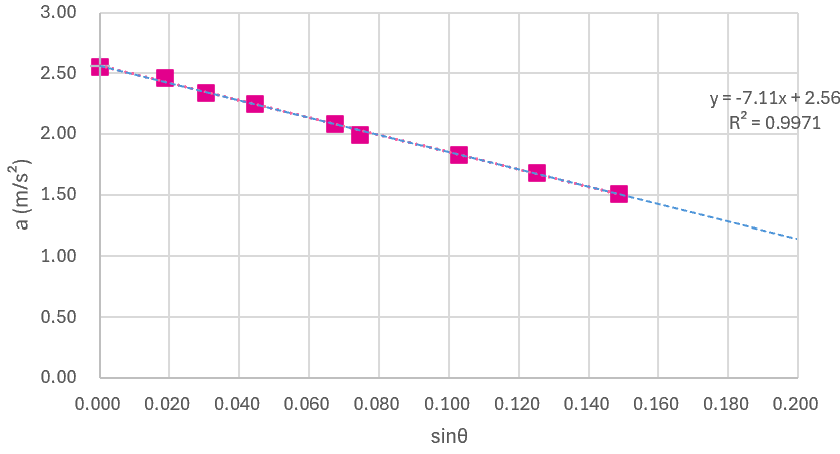
\includegraphics[width=0.8\textwidth]{實驗C數據圖1.png}
                \caption{加速度$a$與$\sin\theta$的關係圖
                }
                \label{fig:實驗C數據圖1}

            \end{figure}

            在 \autoref{fig:實驗C數據圖1}中,粉紅色虛線為實際值趨勢線,藍色虛線為理論值趨勢線,其關係式如下:
            \begin{equation}
                a = \frac{-m_1 g \sin\theta + m_2 g}{m_1 + m_2 + m_{eff}} \label{eq:theory_C1}
            \end{equation}
            由回歸直線得知 $a$ 和 $\sin{\theta}$ 為線性關係,並由回歸直線斜率得 $\displaystyle\frac{-m_1g}{m_1+m_2+m_{eff}}$ = \SI{-7.11},截距得$\displaystyle\frac{m_2g}{m_1+m_2+m_{eff}} = $\SI{2.56}{\meter\per\second\squared}

            \begin{figure}[H]
                
                \centering
                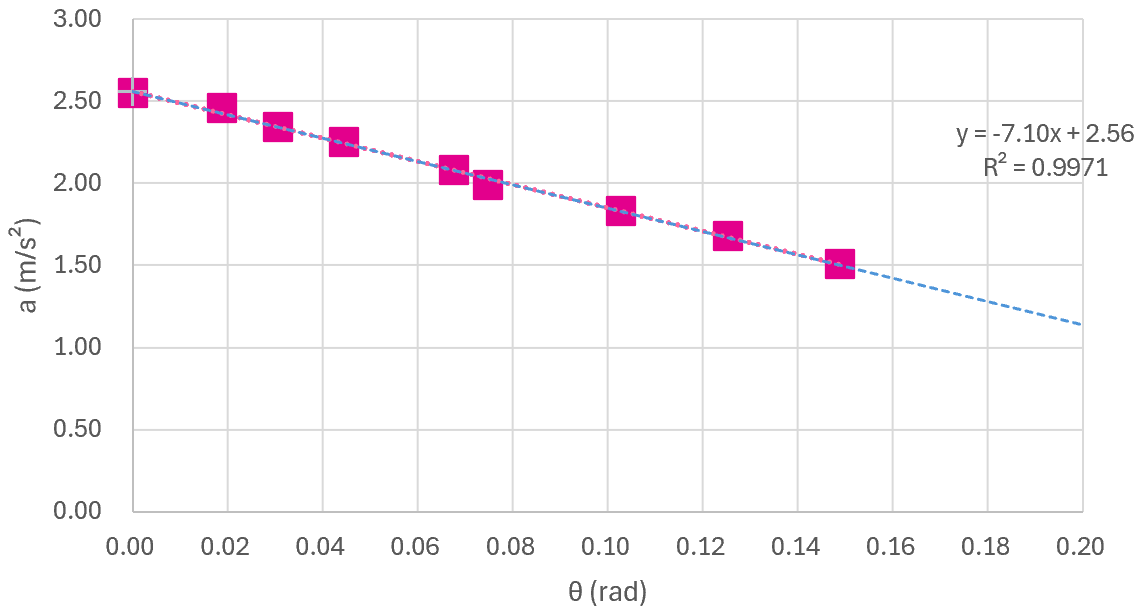
\includegraphics[width=0.8\textwidth]{實驗C數據圖2.png}
                \caption{加速度$a$與$\theta$的關係圖
                }
                \label{fig:實驗C數據圖2}

            \end{figure}

            在 \autoref{fig:實驗C數據圖2}中,粉紅色虛線為實際值趨勢線,藍色虛線為理論值趨勢線,其關係式如下:
            \begin{equation}
                a = \frac{m_1 g \theta + m_2 g}{m_1 + m_2 + m_{eff}} \label{eq:theory_C2}
            \end{equation}
            由回歸直線得知 $a$ 和 $\theta$ 為線性關係,並由回歸直線斜率得 $\displaystyle\frac{-m_1g}{m_1+m_2+m_{eff}}$ = \SI{-7.10},截距得$\displaystyle\frac{m_2g}{m_1+m_2+m_{eff}} = $\SI{2.56}{\meter\per\second\squared}

    \section{討論}

        \subsection{實驗值與理論值之比較}

            \begin{enumerate}
                \item 實驗A
                \par 本實驗中砝碼質量 $m_2 = \SI{0.1461}{\kilogram}$,重力加速度 $g = \SI{9.789}{\meter\per\second\squared}$ \cite{nlsc:twd97}。因此,斜率的理論值計算如下:
                \begin{equation}
                    \frac{1}{m_2 g} = \frac{1}{\SI{0.1461}{\kilogram} \times \SI{9.789}{\meter\per\second\squared}} = \SI{0.6992}{\second\squared\per\kilogram\per\meter}
                \end{equation}
                此理論值與實驗測得的斜率 \SI{0.7204}{\second\squared\per\kilogram\per\meter} 相比,其相對誤差計算如下:

                \begin{equation}
                    \left| \frac{0.7204 - 0.6992}{0.6992} \right| \times 100\% = 3.032\%
                \end{equation}

                \item 實驗B
                \par 經測量本實驗中總質量 $M = m_1 + m_2 + m_{eff} = \SI{0.5345}{\kilogram}$,斜率之理論值

                \begin{equation}
                    \frac{1}{M} = \SI{1.870}{\per\kilogram}
                \end{equation}

                此理論值與實驗測得的斜率\SI{1.860}{\per\kilogram}其相對誤差計算如下:

                \begin{equation}
                    \left| \frac{1.86 - 1.870}{1.870} \right| \times 100\% = 0.535\%
                \end{equation}

                \item 實驗C
                \par 本實驗之$m_1 = \SI{0.3730}{\kilogram}$,$m_2 = \SI{0.1364}{\kilogram}$,其總質量\par$M = \SI{0.3730}{\kilogram} + \SI{0.1364}{\kilogram} = \SI{0.5139}{\kilogram}$,其中斜率之理論值

                \begin{equation}
                    \- \frac{m_1g}{M} = \SI{-7.105}{\meter\per\second\squared} 
                \end{equation}

                此理論值與實驗中以$a$對$\sin{\theta}$作圖測得的斜率\SI{-7.11}{\per\kilogram}其相對誤差計算如下:

                \begin{equation}
                    \left| \frac{-7.11 - (-7.105)}{-7.105} \right| \times 100\% = 0.275\%
                \end{equation}

                與實驗中以$a$對$\theta$作圖測得的斜率\SI{-7.11}{\per\kilogram}其相對誤差計算如下:

                \begin{equation}
                    \left| \frac{-7.10 - (-7.105)}{-7.105} \right| \times 100\% = 0.275\%
                \end{equation}

                而截距之理論值

                \begin{equation}
                    \- \frac{m_2g}{M} = \SI{-2.596}{\meter\per\second\squared} 
                \end{equation}

                此理論值與實驗中以$a$對$\sin\theta$作圖測得的截距\SI{2.56}{\per\kilogram}其相對誤差計算如下:

                \begin{equation}
                    \left| \frac{2.56 - (2.596)}{2.596} \right| \times 100\% = 1.54\%
                \end{equation}

                此理論值與實驗中以$a$對$\theta$作圖測得的截距\SI{2.56}{\per\kilogram}其相對誤差計算如下:

                \begin{equation}
                    \left| \frac{2.56 - (2.596)}{2.596} \right| \times 100\% = 1.54\%
                \end{equation}

            \end{enumerate}

        \subsection{系統性誤差來源}

            \begin{enumerate}

                \item 砝碼擺動
                \par
                雖然實驗時皆有確保砝碼沒有明顯擺動再放開滑車開始實驗,但在手離開砝碼時還是無法避免砝碼晃動。設在滑車未移動時砝碼晃動之高度差為$H = $\SI{0.005}{\meter},砝碼距離滑輪為$r = $\SI{0.1}{\meter},設砝碼在最低點時速度為 $v$,且砝碼可視為簡諧運動。則在最低點時砝碼所需之向心力,即為砝碼晃動對力正偏差比例為

                \begin{equation}
                    \frac{\frac{m_2v^2}{r}}{m_2g} = \frac{2h}{r} \times 100\% = 10\%
                \end{equation}

                雖然實際情況高度差 $H$ 可能因實驗時有盡量更小,且行進中的影響可能也較初始滑車為移動時小,但初步計算可能造成可觀的外力$F$,對加速度$a$造成正偏差。實際上實驗C\ \autoref{fig:實驗C數據圖1} 的$a$對$\sin\theta$作圖和 \autoref{fig:實驗C數據圖2} 的$a$對$\theta$作圖截距較理論值大,即可能砝碼擺動造成額外的加速度所致。

                \item 摩擦力之探討
                \par 滑輪與輪子之摩擦力會阻礙物體運動。雖然沒有精確測量摩擦力,但摩擦力會對加速度$a$造成負偏差,以一般摩擦力和正向力為正比的模型而言,考慮滑車的摩擦力 $m_1 g \cos\theta \mu_k$ ,其中 $\mu_k$ 為滑車和軌道之間的動摩擦力,對 \autoref{fig:實驗A、實驗B示意圖}的實驗B而言,原先的
                
                \begin{equation}
                    a = \frac{F}{m_1 + m_2 + m_{eff}}
                \end{equation}

                可以改寫為

                \begin{equation}
                    a = \frac{F - m_1g\mu
                    }{m_1 + m_2 + m_{eff}}
                \end{equation}

                再將$m_1 = M - m_2 - m_{eff}$、$F = m_2g$帶入

                \begin{equation}
                    a = \frac{F - (M - m_2 - m_{eff})g\mu
                    }{m_1 + m_2 + m_{eff}} = \frac{F(1 + \mu) - (M - m_{eff})g\mu
                    }{m_1 + m_2 + m_{eff}}
                \end{equation}
                

                雖然滑車和軌道之間為純滾動的輪子而非接觸面,此推導仍可能有適性,因為輪軸和輪子之間的正向力正比於滑車和軌道之間的正向力。
                \par
                根據以上推導,使用此模型會造成加速度固定之負偏差,重新分析實驗B加速度$a$對拉力$F$作圖回歸直線:

                \begin{equation}
                    a = \SI{1.86}{\per\kilogram} \times F - \SI{0.0139}{\meter\per\second\squared}
                \end{equation}

                其中$M$ = \SI{0.5345}{\kilogram}。先由截距理論值

                \begin{equation}
                    \frac{(M - m_{eff})g\mu}{m_1 + m_2 + m_{eff}}
                \end{equation}

                得出摩擦係數 $\mu$ = 0.00143。雖然看似略小,但實際上摩擦係數由輪子貢獻,其輪軸經過潤滑,摩擦係數本就應該不大。接著我們使用計算校正後之斜率,由質量理論值搭配算出的摩擦係數計算斜率理論值:

                \begin{equation}
                    \frac{1 + 0.00143}{\SI{0.5345}{\kilogram}} = \SI{1.874}{\per\kilogram}
                \end{equation}

                並和回歸直線斜率之斜率比較

                \begin{equation}
                    \left| \frac{1.86 - 1.870}{1.870} \right| \times 100\% = 0.747\%
                \end{equation}

                故此模型可以解釋實驗B\ \autoref{fig:實驗B數據圖}截距小於0,卻沒有成功解釋斜率的負偏差。
                \par
                前述提到因輪子和滑輪基本上為純滾動,推測摩擦力主要來源為輪軸,而輪軸上有潤滑油,因此摩擦力會包含和速度的正數次方成正比的項,即摩擦力和加速度有正相關。可以解釋實驗A\ \autoref{fig:實驗A數據圖}、實驗B\ \autoref{fig:實驗B數據圖}的斜率小於理論值。
                \par
                另外,在滑車移動的同時,可能輪子可能擦到軌道,造成摩擦力。因此我們在實驗前皆有經過水平儀確認滑車移動時沒有側面方向的傾斜,以降低這種影響。

                \item 滑輪與棉線之相對運動
                \par
                當我們在實驗中用軟體測量滑輪的邊緣速率對時間的斜率,即加速度時,滑車開始移動後時間越長,其加速度稍低。除了摩擦力的影響,推測在滑車運動速率較快時,考慮棉線振動,棉線與滑輪之間有相對運動,即棉線並不會完全貼合滑輪帶動滑輪轉動,造成加速度測量低於理論值。其中一個改進方法為使用摩擦係數更大的滑輪或繩子。
                
            \end{enumerate}

        \subsection{隨機性誤差來源}

            在實驗A、實驗B、實驗C中作圖之 $R^2$ 皆大於0.99,在趨勢上相對穩定。在此列出一些因素並說明是否為誤差來源。
            \begin{enumerate}

                \item 電子秤本身之測量誤差
                \par
                實驗中所測量之質量皆大於 \SI{0.05}{\kilogram},而電子秤之最小位數為\SI{0.0001}{\kilogram},誤差小於 $\displaystyle\frac{1}{500}$,遠小於實驗A、實驗C的誤差,但和實驗B之誤差 0.275\% 為同個數量級,可能為誤差來源。
                \item 直尺測量之誤差
                \par
                用於實驗C測量高度之直尺最小刻度為\SI{0.001}{\meter},其B類不確定度為\SI{0.00029}{\meter}。而對於實驗C所計算之$h_1 - h_2$因誤差傳遞,不確定度為\SI{0.00058}{\meter}。而$h_1 - h_2$之部分數據為\SI{e-3}{\meter}等級,其不確定度高達數值5\%,但因為大部份數據之$h_1 - h_2$為\SI{e-2}{\meter},故影響較小。
            \end{enumerate}

        \subsection{可忽略之誤差}

            \begin{enumerate}

                \item $\theta$ 近似之誤差
                \par
                在實驗C中,$\theta$ 最大約為 \ang{8.5} < \ang{10},故將 $\sin{\theta}$ 近似為$\theta$ 為有效近似。所以比較實驗C的 \autoref{fig:實驗C數據圖1} 的$a$對$\sin\theta$作圖和 \autoref{fig:實驗C數據圖2} 的$a$對$\theta$作圖幾乎沒有區別。

                \item 棉線質量
                \par
                實驗中無足夠精準之儀器或足夠長的棉線測量棉線質量,但一般棉線之線密度約為$\SI{e-4}{} \sim \SI{e-5}{\kilogram\per\meter}$ 而本實驗之物體總質量皆大於 \SI{0.3}{\kilogram},棉線長度約 $\SI{1}{} \sim \SI{2}{\meter}$,故誤差小於0.067\%,遠小於實驗A、實驗B、實驗C之誤差。

                \item 光閘測量加速度誤差
                \par
                在實驗中使用 Capstone 測量軟體時,取到的速度數據形成之回歸直線 $R^2$ 皆大於 0.99,且不確定度皆為 \SI{e-10}{\meter\per\second\squared}以下數量級,故光閘之測量誤差可以忽略。

            \end{enumerate}

        \subsection{其他誤差討論}

            \begin{enumerate}

                \item 回歸直線中截距的誤差
                \par
                實驗C 中\ \autoref{fig:實驗C數據圖1}\ 和\ \autoref{fig:實驗C數據圖2},可能是因為回歸直線中截距為相減的結果,較難保證其準確性。但我們仍將實驗C兩張圖的截距的誤差控制在1.5\%,而實驗A中\ \autoref{fig:實驗A數據圖}\ 和實驗B中\ \autoref{fig:實驗B數據圖} 的截距不大,而使變數之間明顯符合正比關係。

            \end{enumerate}

    \section{結論}
        本實驗進行的三項實驗結果皆相當接近,並足以支持牛頓第二運動定律。而砝碼擺動、摩擦力、電子秤、直尺為潛在的誤差來源。
    \nocite{*}
    \printbibliography[title={參考資料}]

    \section*{附錄}
        \begin{enumerate}
            \item 實驗A原始數據
            \begin{figure}[H]
                
                \centering
                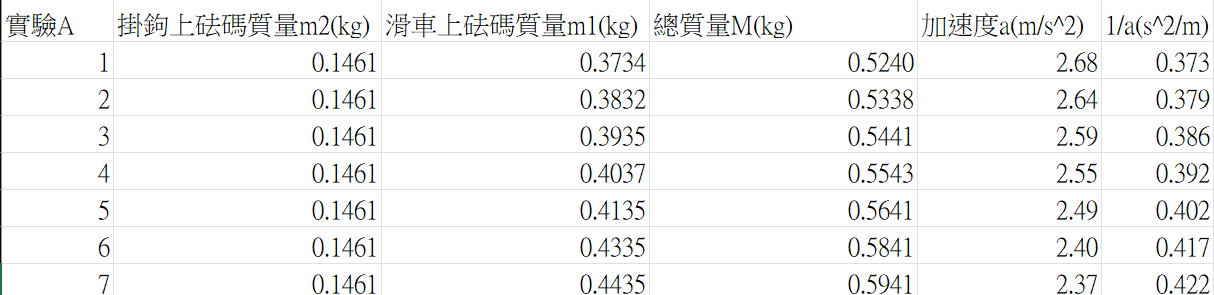
\includegraphics[width=0.8\textwidth]{實驗A原始數據.png}
                \caption{實驗A Excel原始數據}
                \label{fig:實驗A Excel原始數據}

            \end{figure} 
            \item 實驗B原始數據
            \begin{figure}[H]
                
                \centering
                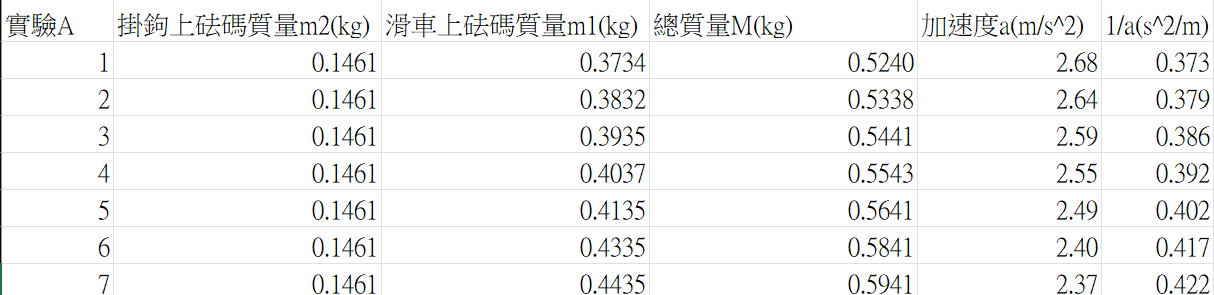
\includegraphics[width=0.8\textwidth]{實驗B原始數據.png}
                \caption{實驗B Excel原始數據}
                \label{fig:實驗B Excel原始數據}

            \end{figure}
            \item 實驗C原始數據
            \begin{figure}[H]
                
                \centering
                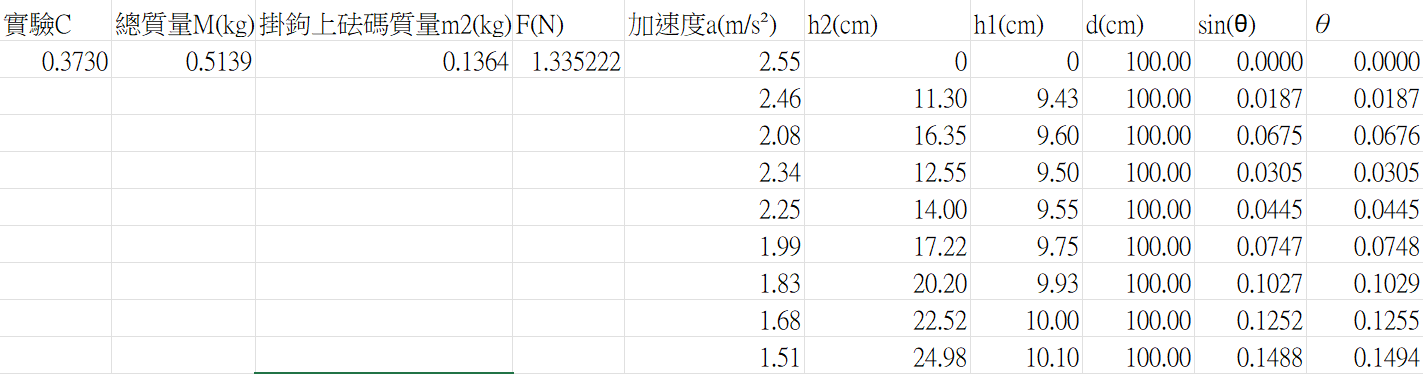
\includegraphics[width=0.8\textwidth]{實驗C原始數據.png}
                \caption{實驗C Excel原始數據}
                \label{fig:實驗C Excel原始數據}

            \end{figure} 
        \end{enumerate}
\end{document}
\displaystyle